% appendices


\chapter{Resynthesizing Audio from Spectrograms}
\label{appendix_resynth}




% \clearpage
% \chapter{correccted}

The \gls{ssast} is trained on Mel spectrograms, which are 2-dimensional representations of the frequencies present in an audio sample. The columns in a spectrogram are derived from the amplitude response, i.e. the absolute value of the Fourier transform (Equation \ref{eq:power_spectrum}). This process results in the loss of phase information. To resynthesize the raw audio signal from its spectrogram, the phase must be estimated, which can be done using the Griffin-Lim algorithm \cite{Griffin1983SignalEF}. Although there is no implementation for \textit{Mel} spectrograms in torchaudio, the librosa library offers this functionality in a feature inversion function called \href{https://librosa.org/doc/main/generated/librosa.feature.inverse.mel_to_audio.html}{\texttt{mel\_to\_audio}} \cite{McFee2015librosaAA}.

However, there are notable differences in the Mel spectrograms calculated by the two libraries for the same audio file. Mel spectrograms from torchaudio default to a $\log_e$ scale, which is the scale used in the original training of the \gls{ssast}. In contrast, the feature inversion function of librosa expects the spectrogram to be on a linear scale. Additionally, as described in Section \ref{sec:mel_spectrogram_conversion}, torchaudio applies a pre-emphasis filter (Equation \ref{eq:preemphasis}), but librosa does not. To mitigate these differences, a custom function, described below, was implemented.

Given a Mel spectrogram to be resynthesized, $X \in \mathbb{R}^{M \times L}$, and a reference audio signal $s_{\text{reference}} \in \mathbb{R}^l$, the function \href{https://github.com/Ironmomo/SpeakerVerificationBA/blob/master/plots_and_audios/audios_thesis.ipynb}{\texttt{synthesize\_audio\_from\_spectrogram}} performs the following operations:

First, it computes the Mel spectrogram of the reference signal $s_{\text{reference}}$ using both librosa's \href{https://librosa.org/doc/main/generated/librosa.feature.melspectrogram.html}{\texttt{melspectrogram}} function ($\rightarrow X_{\text{librosa}}$) and torchaudio's Kaldi-compliant \href{https://pytorch.org/audio/main/generated/torchaudio.compliance.kaldi.fbank.html}{\texttt{fbank}} function ($\rightarrow X_{\text{torchaudio}}$). The resulting spectrograms are then transformed to the dB scale.

Next, an additive transformation aligns the spectrogram computed by torchaudio, $X_{\text{torchaudio}}$, with that computed by librosa, $X_{\text{librosa}}$. This is achieved by adding a polynomial function $p(f)$,
\begin{equation}
    p(f) := \sum_{i=0}^{n} c_i f^i,
\end{equation}
to each frame of $X_{\text{torchaudio}}$ to minimize the difference:
\begin{equation}
   \Delta X(f, t) := X_{\text{librosa}}(f, t) - X_{\text{torchaudio}}(f, t). 
\end{equation}

The polynomial $p(f)$ is fitted by solving a least squares problem:
\begin{equation}
c = \text{argmin}_c ||\Delta X(f, t) - p(f)||^2,
\end{equation}
where $f$ is the Mel frequency bin index, $t$ is the time frame index, $n$ is the order of the polynomial, and $c_i$ are the coefficients of the polynomial.

The coefficient vector $c \in \mathbb{R}^{n+1}$ can be calculated by solving the normal equation:
\begin{equation}
A^T A c = A^T b \Rightarrow c = (A^T A)^{-1} A^T b
\end{equation}
where $A \in \mathbb{R}^{(M \cdot L) \times (n+1)}$ is the matrix of polynomial features and $b \in \mathbb{R}^{M \cdot L}$ is the (flattened) vector of differences between the two Mel spectrograms.

The polynomial $p(f)$ is then applied to the Mel spectrogram to be synthesized, $X(f, t)$, to account for the differences between the two libraries:
\begin{equation}
X_{\text{adjusted}}(f, t) = X(f, t) + p(f)
\end{equation}
Figure \ref{fig:resynthesis_adjustments} shows this process for a cross section (one frame/column) of a spectrogram.

Finally, the adjusted Mel spectrogram is transformed back to a linear scale and synthesized into audio using the feature inversion function \href{https://librosa.org/doc/main/generated/librosa.feature.inverse.mel_to_audio.html}{\texttt{mel\_to\_audio}} from the librosa library.

\begin{figure}[H]
    \centering
    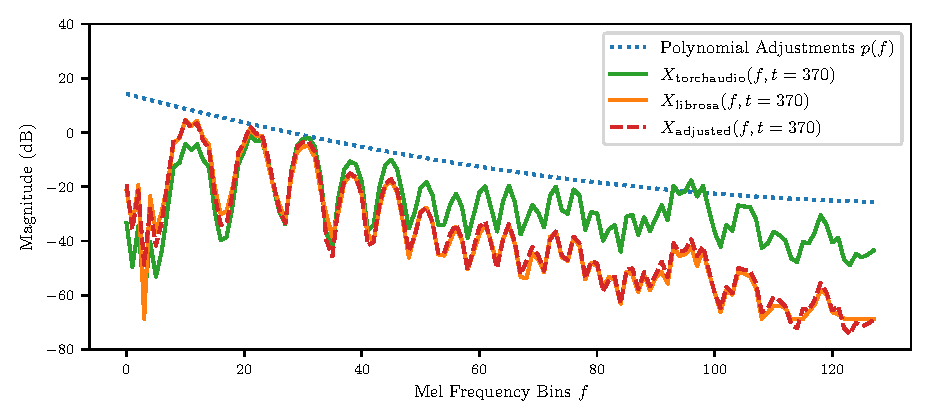
\includegraphics[width=1\linewidth]{img/plots/resynthesis_adjustments.pdf}
    \caption{Illustration of the polynomial adjustments $p(f)$ calculated from the difference between the Mel spectrograms of the reference audio signal (blue, dotted). Additionally, a cross-section of the Mel spectrograms at the $370^{\text{th}}$ time frame is shown.}
    \label{fig:resynthesis_adjustments}
\end{figure}












\clearpage
\chapter{More Resynthesized Spectrograms}\label{appendix_resynth_examples}

This appendix contains further examples of the pretrained model (trained on original data) reconstructing spectrograms. Figure \ref{fig:speech_reconstruction} and \ref{fig:music_reconstruction} contain $N=180$ manually constructed mask indices which translate to a time duration of 3.6 seconds in total. Each mask has an extent/width of 20 frame-like patches, which corresponds to 0.4 seconds of audio.

\begin{figure}[htbp]
    \centering
    \begin{tikzpicture}
        \node[anchor=south west,inner sep=0] (image) at (0,0) {
            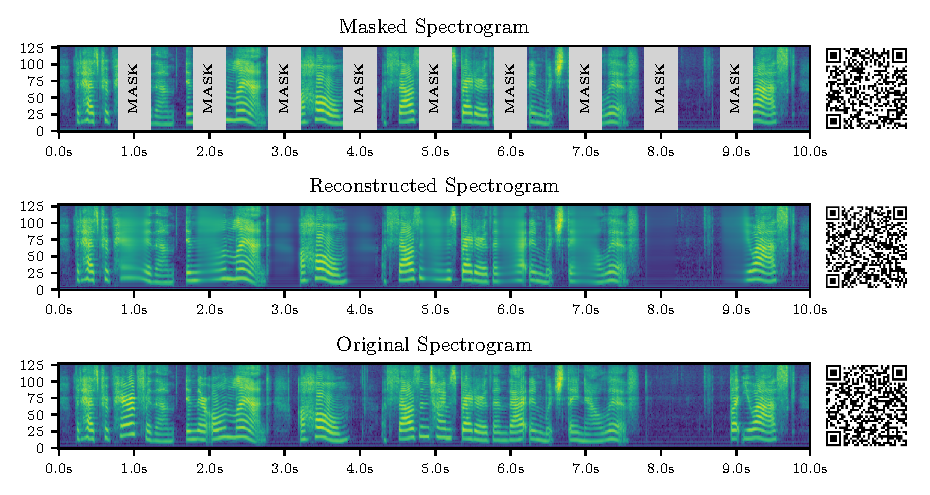
\includegraphics[width=1\linewidth]{img/plots/reconstructed_spectrogram_speech.pdf}
        };
        
        % Define the scope for the image size
        \begin{scope}[x={(image.south east)},y={(image.north west)}]
            % Define clickable areas
            \node at (0.93,0.81875) {                \href{https://github.com/Ironmomo/SpeakerVerificationBA/raw/master/plots_and_audios/audios/masked_speech.wav}{
                    \tikz{\path[fill=none] (0,0) rectangle (0.07,0.165);}
                }
            };
            \node at (0.93,0.5) {                \href{https://github.com/Ironmomo/SpeakerVerificationBA/raw/master/plots_and_audios/audios/reconstructed_speech.wav}{
                    \tikz{\path[fill=none] (0,0) rectangle (0.07,0.165);}
                }
            };
            \node at (0.93,0.18125) {                \href{https://github.com/Ironmomo/SpeakerVerificationBA/raw/master/plots_and_audios/audios/original_speech.wav}{
                    \tikz{\path[fill=none] (0,0) rectangle (0.07,0.165);}
                }
            };
        \end{scope}
    \end{tikzpicture}
    \caption{Reconstructing the same spectrogram as in Figure \ref{fig:originalModel_spectrogramReconstruction} and \ref{fig:shuffledModel_spectrogramReconstruction}, but using a manually chosen set $I$ of masked indices. Resynthesized audio files from each spectrogram can be downloaded by clicking or scanning the corresponding QR-Code.}
    \label{fig:speech_reconstruction}
\end{figure}

The sample that was used for Figure \ref{fig:speech_reconstruction} is the same that was already used in Figure \ref{fig:originalModel_spectrogramReconstruction} and \ref{fig:shuffledModel_spectrogramReconstruction}. Figure \ref{fig:music_reconstruction} shows the reconstruction of a spectrogram of music. The longest trained models (trained for 10 epochs / 428k Iterations), seems to have a quite accurate sense of melody and rhythm.

Figure \ref{fig:speech_reconstruction_longmask} shows a masked spectrogram with one large mask of 1.6 seconds at the center of the spectrogram. As can be seen in the \textit{Reconstructed Spectrogram from Original Model}, even the model trained on original spectrograms tends to make something resembling the average, if a masked patch has a large width.

% \newgeometry{top=1.0in}
\begin{figure}[h]
% \vspace{-2pt}
    \centering
    \begin{tikzpicture}
    % \settowidth{\imagewidth}{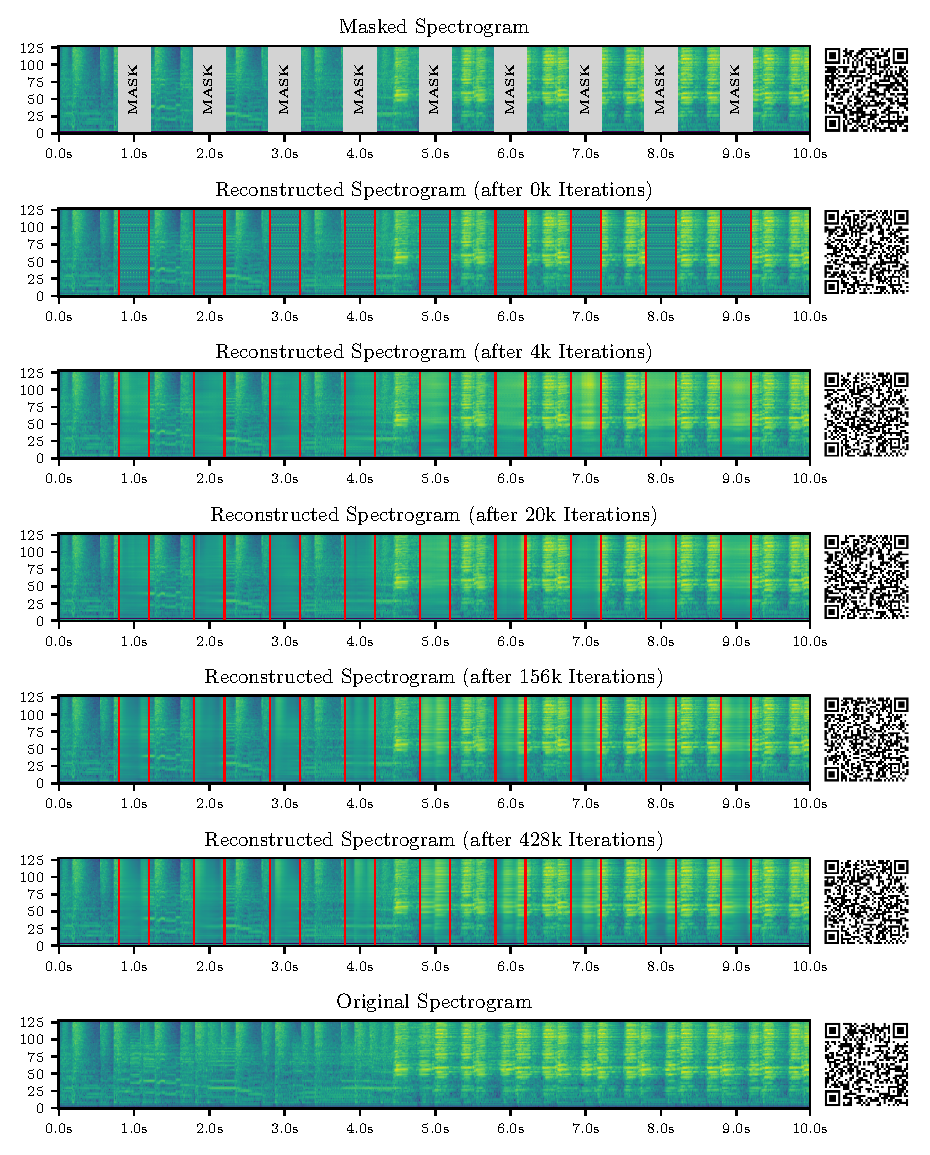
\includegraphics{img/plots/reconstructed_spectrogram_music.pdf}}
    % \settoheight{\imageheight}{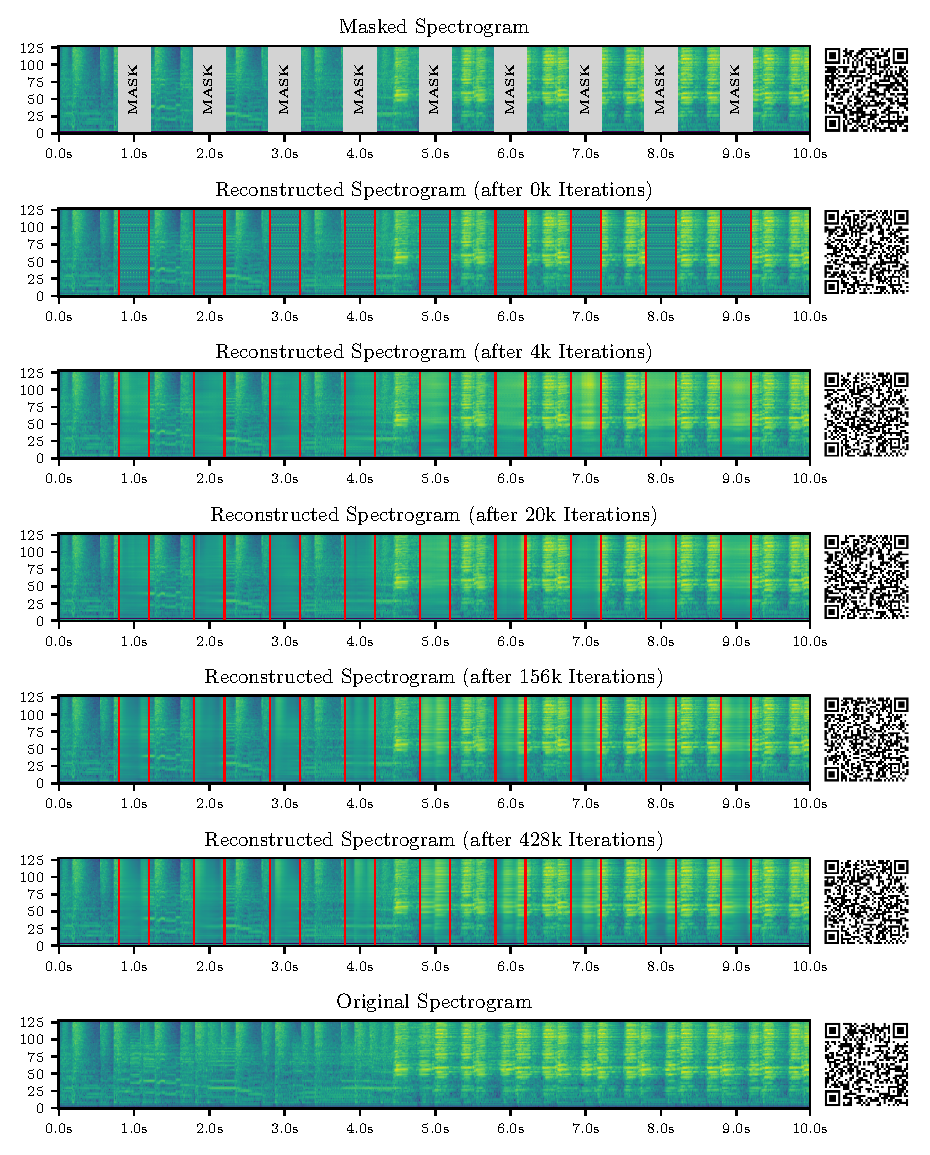
\includegraphics{img/plots/reconstructed_spectrogram_music.pdf}}
    %     \node[anchor=south west,inner sep=0] (image) at (0,0) {
    %         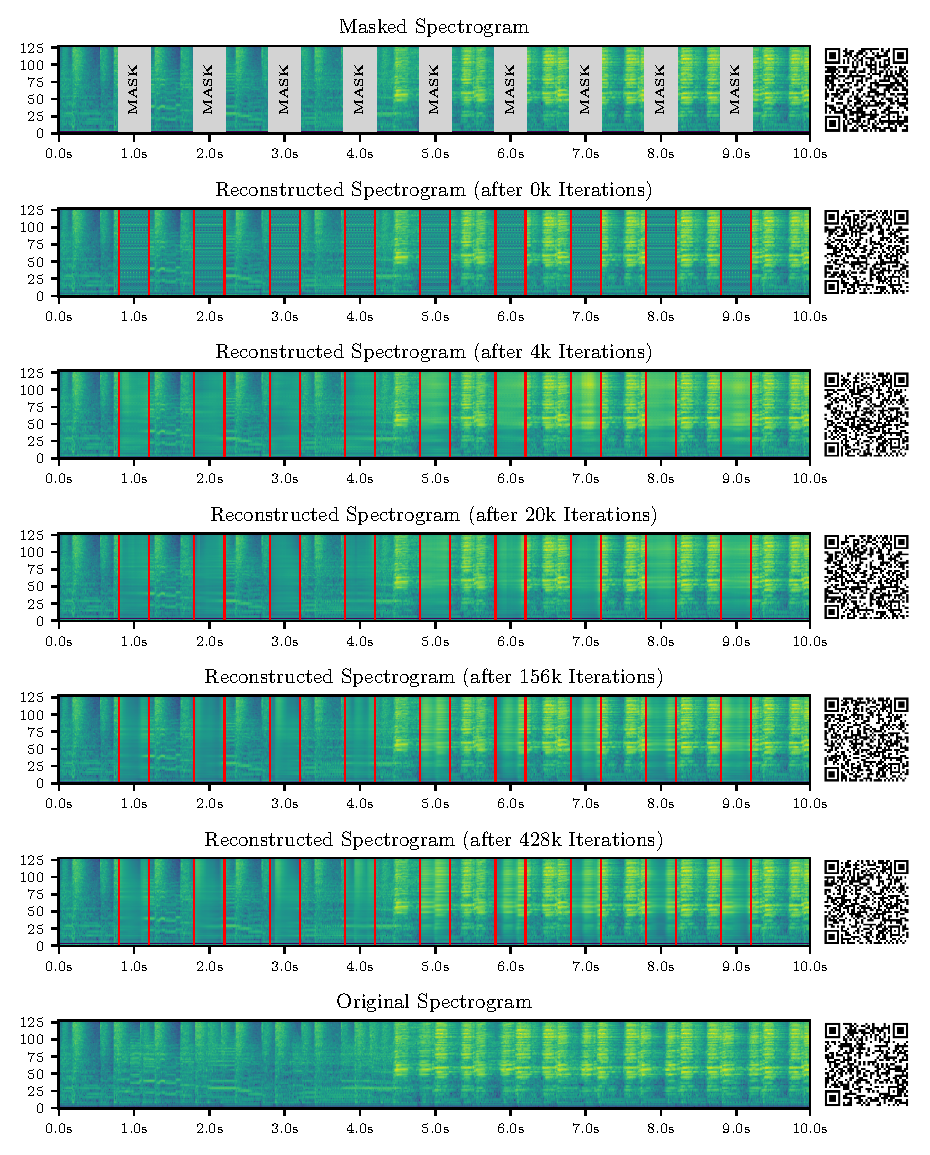
\includegraphics[width=1\linewidth, clip, viewport=0 0.01\imageheight{} \imagewidth{} 0.99\imageheight{}]{img/plots/reconstructed_spectrogram_music.pdf}
    %     };
        \node[anchor=south west,inner sep=0] (image) at (0,0) {
            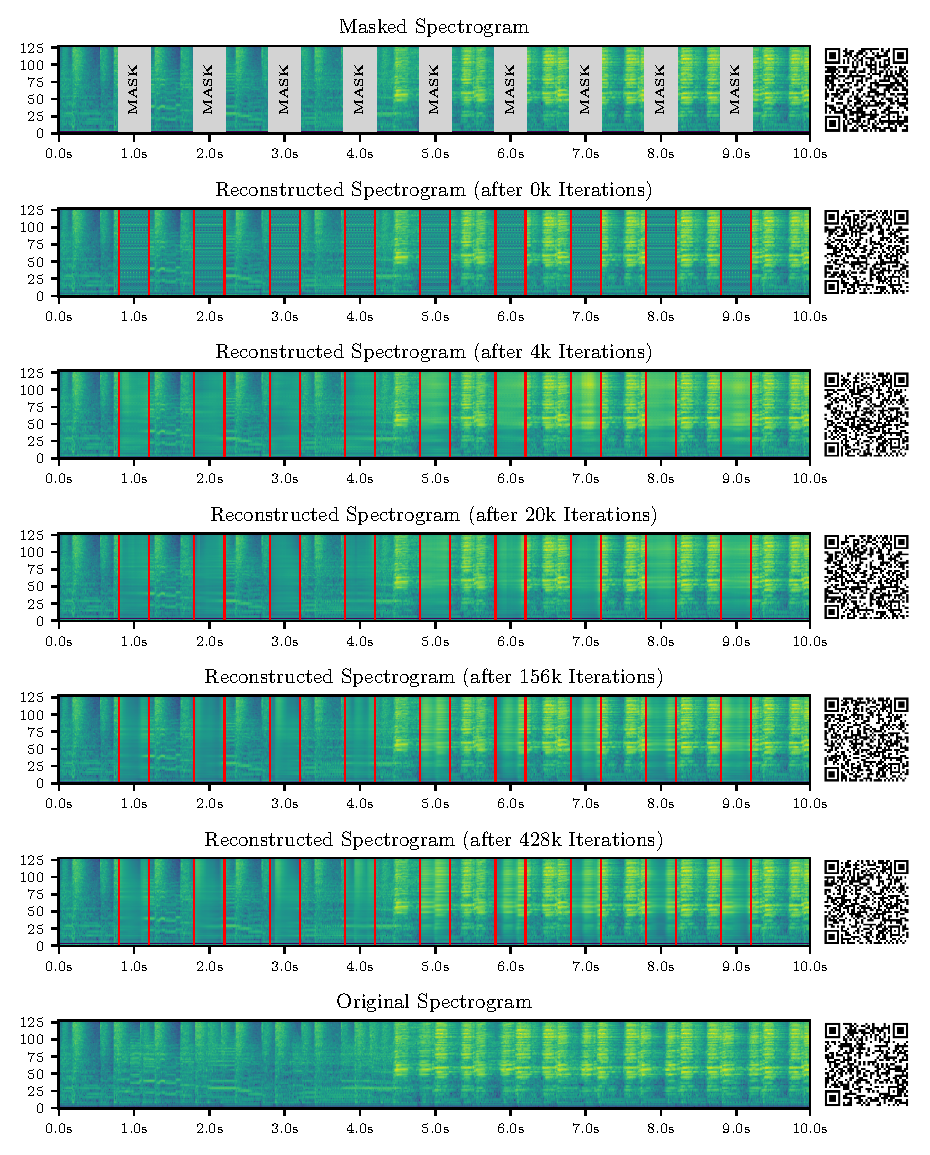
\includegraphics[width=1\linewidth]{img/plots/reconstructed_spectrogram_music.pdf}
        };
        
        % Define the scope for the image size
        \begin{scope}[x={(image.south east)},y={(image.north west)}]
            % Define clickable areas
            \node at (0.93,0.08+6.0/7.1) {                \href{https://github.com/Ironmomo/SpeakerVerificationBA/raw/master/plots_and_audios/audios/masked_music.wav}{
                    \tikz{\path[fill=none] (0,0) rectangle (0.07,0.07);} % (x, y) ≙ (width, height)
                }
            };
            \node at (0.93,0.08+5.0/7.1) {                \href{https://github.com/Ironmomo/SpeakerVerificationBA/raw/master/plots_and_audios/audios/reconstructed_music_1.wav}{
                    \tikz{\path[fill=none] (0,0) rectangle (0.07,0.07);}
                }
            };
            \node at (0.93,0.08+4.0/7.1) {                \href{https://github.com/Ironmomo/SpeakerVerificationBA/raw/master/plots_and_audios/audios/reconstructed_music_2.wav}{
                    \tikz{\path[fill=none] (0,0) rectangle (0.07,0.07);}
                }
            };
            \node at (0.93,0.08+3.0/7.1) {                \href{https://github.com/Ironmomo/SpeakerVerificationBA/raw/master/plots_and_audios/audios/reconstructed_music_6.wav}{
                    \tikz{\path[fill=none] (0,0) rectangle (0.07,0.07);}
                }
            };
            \node at (0.93,0.08+2.0/7.1) {                \href{https://github.com/Ironmomo/SpeakerVerificationBA/raw/master/plots_and_audios/audios/reconstructed_music_40.wav}{
                    \tikz{\path[fill=none] (0,0) rectangle (0.07,0.07);}
                }
            };
            \node at (0.93,0.08+1.0/7.1) {                \href{https://github.com/Ironmomo/SpeakerVerificationBA/raw/master/plots_and_audios/audios/reconstructed_music_108.wav}{
                    \tikz{\path[fill=none] (0,0) rectangle (0.07,0.07);}
                }
            };
            \node at (0.93,0.08) {                \href{https://github.com/Ironmomo/SpeakerVerificationBA/raw/master/plots_and_audios/audios/original_music.wav}{
                    \tikz{\path[fill=none] (0,0) rectangle (0.07,0.07);}
                }
            };
        \end{scope}
    \end{tikzpicture}
    % \captionsetup{aboveskip=0pt, belowskip=-55pt}
    \caption{Reconstructing a spectrogram of music with the model at different stages of pretraining. Resynthesized audio files from each spectrogram can be downloaded by clicking or scanning the corresponding QR-Code.}
    \label{fig:music_reconstruction}
\end{figure}
\clearpage
% \restoregeometry



\begin{figure}[htbp]
    \centering
    \begin{tikzpicture}
        \node[anchor=south west,inner sep=0] (image) at (0,0) {
            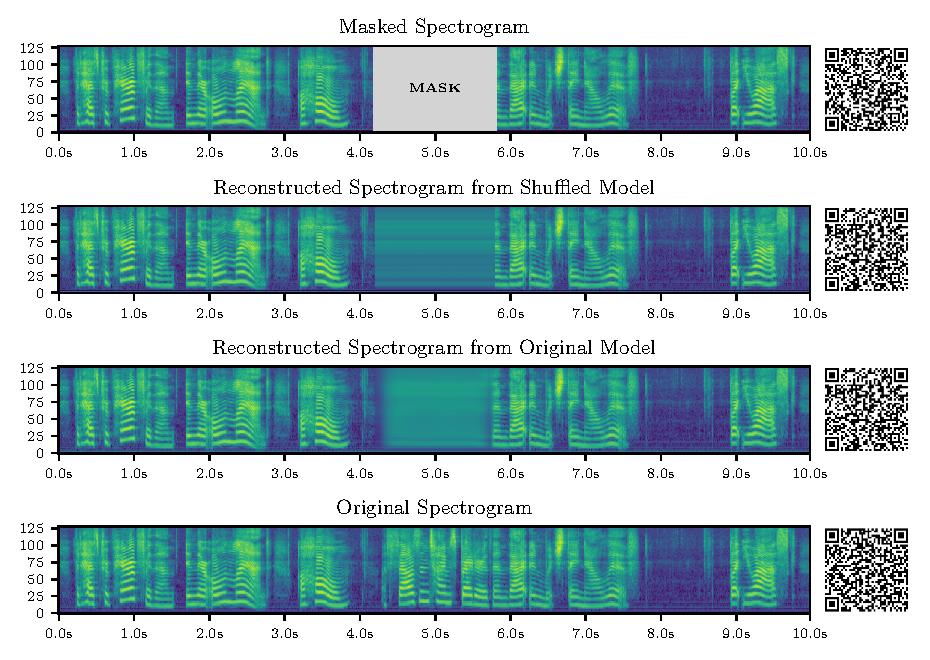
\includegraphics[width=1\linewidth]{img/plots/reconstructed_spectrogram_speech_longmask.pdf}
        };
        
        % Define the scope for the image size
        \begin{scope}[x={(image.south east)},y={(image.north west)}]
            % Define clickable areas
            \node at (0.93,0.138+3*0.242) {                \href{https://github.com/Ironmomo/SpeakerVerificationBA/raw/master/plots_and_audios/audios/masked_speech_longmask.wav}{
                    \tikz{\path[fill=none] (0,0) rectangle (0.07,0.12);}
                }
            };
            \node at (0.93,0.138+2*0.242) {                \href{https://github.com/Ironmomo/SpeakerVerificationBA/raw/master/plots_and_audios/audios/reconstructed_speech_SUModel_longmask.wav}{
                    \tikz{\path[fill=none] (0,0) rectangle (0.07,0.12);}
                }
            };
            \node at (0.93,0.138+0.242) {                \href{https://github.com/Ironmomo/SpeakerVerificationBA/raw/master/plots_and_audios/audios/reconstructed_speech_OSModel_longmask.wav}{
                    \tikz{\path[fill=none] (0,0) rectangle (0.07,0.12);}
                }
            };
            \node at (0.93,0.138) {                \href{https://github.com/Ironmomo/SpeakerVerificationBA/raw/master/plots_and_audios/audios/original_speech.wav}{
                    \tikz{\path[fill=none] (0,0) rectangle (0.07,0.12);}
                }
            };
        \end{scope}
    \end{tikzpicture}
    \caption{Manually masking $N=80$ of the frame-like $2 \times 128$ patches, but aligning the masks all at the center and next to each other, forming one large mask of 1.6 seconds. Resynthesized audio files from each spectrogram can be downloaded by clicking or scanning the corresponding QR-Code.}
    \label{fig:speech_reconstruction_longmask}
\end{figure}
